\documentclass[10pt]{beamer}
\usetheme[%%% option passed to the outer theme
%    progressstyle=fixedCircCnt,   % fixedCircCnt, movingCircCnt (moving is deault)
 ]{Feather}

% If you want to change the colors of the various elements in the theme, edit and uncomment the following lines

% Change the bar colors:
%\setbeamercolor{Feather}{fg=red!20,bg=red}

% Change the color of the structural elements:
%\setbeamercolor{structure}{fg=red}

% Change the frame title text color:
%\setbeamercolor{frametitle}{fg=blue}

% Change the normal text color background:
%\setbeamercolor{normal text}{fg=black,bg=gray!10}

%-------------------------------------------------------
% INCLUDE PACKAGES
%-------------------------------------------------------

\usepackage[utf8]{inputenc}
\usepackage[english]{babel}
\usepackage[T1]{fontenc}
\usepackage{helvet}
\usepackage{algorithm, algpseudocode}
\usepackage{graphicx,psfig,amsmath,float,epstopdf,multirow,mathtools,changepage,amssymb}
\usepackage[para,online,flushleft]{threeparttable}
%-------------------------------------------------
\usepackage{float} % lets you have non-floating floats
\usepackage{url} % for typesetting urls
\usepackage{caption}
\usepackage{program}
\usepackage{tabularx}
\usepackage{colortbl}
\usepackage{etoolbox}
\usepackage{hhline}
\usepackage{subcaption}
\usepackage{amsmath}
\let\bbordermatrix\bordermatrix
%\patchcmd{\bbordermatrix}{8.75}{4.75}{}{}
%\patchcmd{\bbordermatrix}{\left(}{\left[}{}{}
%\patchcmd{\bbordermatrix}{\right)}{\right]}{}{}]})}

% DEFFINING AND REDEFINING COMMANDS
%-------------------------------------------------------

% colored hyperlinks
\newcommand{\chref}[2]{
  \href{#1}{{\usebeamercolor[bg]{Feather}#2}}
}

%-------------------------------------------------------
% INFORMATION IN THE TITLE PAGE
%-------------------------------------------------------

\title[] % [] is optional - is placed on the bottom of the sidebar on every slide
{ % is placed on the title page
      \textbf{QOS AWARE WEB SERVICE DISTRIBUTION DESIGN}
}

%\subtitle[The Feather Beamer Theme]
%{
      %\textbf{v. 1.0.0}
%}

\author[Boxiong Tan]
{      Boxiong Tan\\
		Supervisors: Hui Ma, Mengjie Zhang\\
      %{\ttfamily lilqna.v@gmail.com}
}

\institute[]
{
      Victoria University of Wellington\\
  
  %there must be an empty line above this line - otherwise some unwanted space is added between the university and the country (I do not know why;( )
}

\date{\today}

%-------------------------------------------------------
% THE BODY OF THE PRESENTATION
%-------------------------------------------------------

\begin{document}

%-------------------------------------------------------
% THE TITLEPAGE
%-------------------------------------------------------

{\1% % this is the name of the PDF file for the background
\begin{frame}[plain,noframenumbering] % the plain option removes the header from the title page, noframenumbering removes the numbering of this frame only
  \titlepage % call the title page information from above
\end{frame}}


%\begin{frame}{Introduction}{}
%\tableofcontents
%\end{frame}

%-------------------------------------------------------
\section{Introduction}
%-------------------------------------------------------
\subsection{Web service Location-Allocation Problem Modeling}
\subsection{Develop a Multi-Objective PSO based approach}
\begin{frame}{Introduction}{}
%-------------------------------------------------------

%\begin{block}{Motivation}
	Web service providers want to find a way to maximize their profit as well as improve the quality of services.
%\end{block}

Main goals:
\begin{itemize}
	\item Minimize the total cost 
	\item Maximize the quality of services
\end{itemize}

\hfill

A promising approach to solve this problem is to allocate services
across multiple locations. Unfortunately, it is \textbf{NP-hard} to find an optimal plan when consider
multiple-factors.

	\begin{itemize}
		\item Single objective algorithms: Linear programming $\rightarrow$ Low efficiency
		\item Multi-objective genetic algorithm (NSGA-II) $\rightarrow$ Low scalability
	\end{itemize}


	\hfill


\end{frame}

\begin{frame}{Project Aims}

PSO has shown its promise in solving NP-hard problem.

\hfill

The aim of this project is to propose a multi-objective PSO based algorithm to solve this problem.

\begin{itemize}
    \item To model the Web service location-allocation problem
    \item To develop a Multi-objective PSO based approach
  \end{itemize}
\end{frame}

%-------------------------------------------------------
\section{Work Done}
%-------------------------------------------------------
\subsection{Problem Modeling}
%\begin{frame}{Work Done}{Problem Modeling}
%-------------------------------------------------------
%\begin{block}{}
%The theme contains 4 source files:
  %\begin{itemize}
    %\item {\tt beamercolorthemeFeather.sty}
    %\item {\tt beamerouterthemeFeather.sty}
    %\item {\tt beamerinnerthemeFeather.sty}
    %\item {\tt beamerthemeFeather.sty}
  %\end{itemize}
%\end{block}

%Main factors that affect the location-allocation decision:
%\begin{itemize}
	%\item Network latency: a key measurement of service quality
	%\item Service invocation frequency: denotes the popularity of a service
	%\item Deployment cost: major cost that we consider
%\end{itemize}
%
%We modelled the input data as a matrix representation.
%
%Example: Cost matrix
%In this paper, we will use the following matrices.
%\begin{center}
	%{
		%%\centering
		%\begin{tabular}{l*{2}{l}r}
			%\hline
			%\textbf{Matrices} \cr
			%$L$ & server network latency matrix $L = \{l_{ij}\}$ \cr
			%$A$ & service location-allocation matrix $A = \{a_{sj}\}$ \cr
			%%$A'$ & service location matrix $A' = \{a'_{sj}\}$ \cr
			%$F$ & service invocation frequency matrix $F = \{f_{is}\}$ \cr
			%$C$ & cost matrix $C = \{c_{sj}\}$ \cr
			%$R$ & user response time matrix $R = \{r_{is}\}$ \cr
			%\hline
		%\end{tabular}
		%%\\
	%}
%\end{center}

%\parbox{.45\linewidth}{
	%{\centering
		%$
		%C = \bbordermatrix{~ & j_{1} & j_{2} & j_{3}\cr
		%s_{1}	&130 &80 &60\cr
		%s_{2}	&96  &52 &86\cr
	%s_{3}	&37 &25 &54\cr}
		%$
	%\\}
%}
%\parbox{.45\linewidth}{
	%{\centering
		%$
		%A = \bbordermatrix{~ & j_{1} & j_{2} & j_{3}\cr
		%s_{1}	&0 &1 &0	\cr
		%s_{2}	&0  &0 &1	\cr
	%s_{3}	&1 &1 &0	\cr}
		%$
	%\\}
%}


%\end{frame}

%-------------------------------------------------------
\subsection{Algorithm Design}
\begin{frame}{Work Done}{Problem Modeling}

%Particle Representation:
%$
%A' = \bbordermatrix{~ & j_{1} & j_{2} & j_{3}\cr
				%s_{1}	&0.12 &0.87 &0.42	\cr
				%s_{2}	&0.07  &0.32 &0.95	\cr
				%s_{3}	&0.76 &0.64 &0.27	\cr}
%$
Factors that affect the decision making.
\begin{figure}
	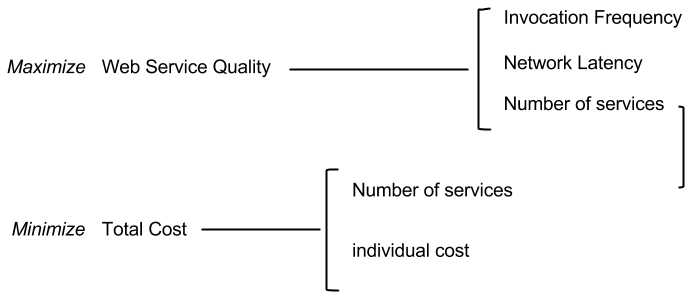
\includegraphics[width=\textwidth]{./Feathergraphics/factors.png}
\end{figure}


%Two fitness functions. 
	%\begin{equation}
		%\resizebox{.4\hsize}{!}{
		%LatencyFitness = \sum\limits_{i \in I} \sum\limits_{s \in S} r_{is} \times f_{is}
	%}
	%\end{equation}

	%\begin{equation}
		%\resizebox{.4\hsize}{!}{
		%CostFitness = \sum\limits_{s \in S} \sum\limits_{j \in J} c_{sj} \times a_{sj}
	%}
	%\end{equation}

	
	%-------------------------------------------------------Design

%Problem Modeling
  %The theme can be installed for \textbf{local} or \textbf{global} use.
  %\pause
  %\begin{block}{Local Installation}
  %\begin{itemize}    
    %\item Local installation is the simplest way of installing the theme. 
    %\item You need to placing the 4 source files in the same folder as your presentation. When you download the theme, the 4 theme files are located in the {\tt local} folder.
  %\end{itemize}
  %\end{block}

  %\begin{block}{Global Installation}
  %\begin{itemize}
     %\item If you wish to make the theme globally available, you must put the files in your local latex directory tree. The location of the root of the local directory tree depends on your operating system and the latex distribution. 
     %\item Detailed steps on how to proceed installation under various operating systems can be found at Beamer documentation.
  %\end{itemize}
  %\end{block}
\end{frame}
     


\begin{frame}{Work Done}{Modeling Details}

Fitness functions:
\begin{figure}
	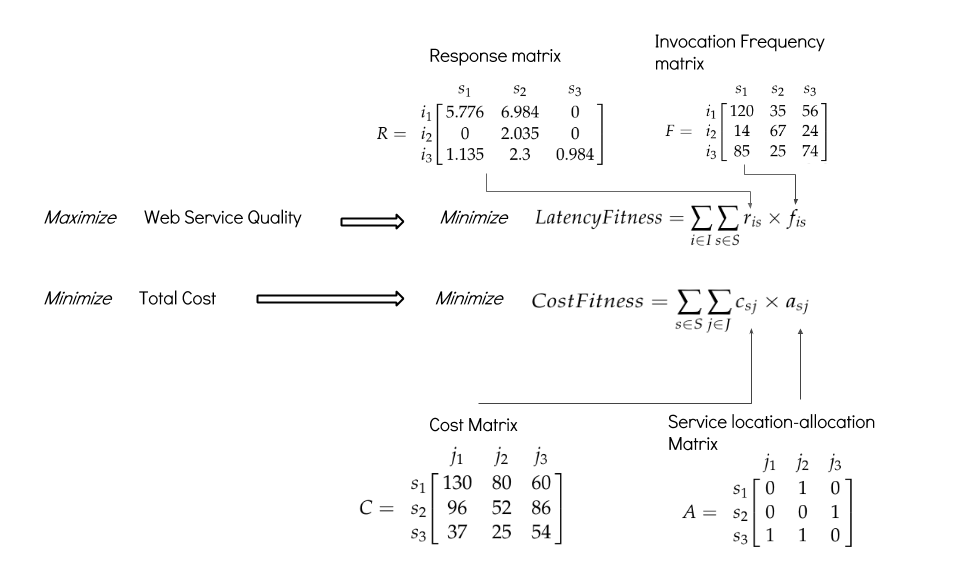
\includegraphics[width=\linewidth]{./Feathergraphics/state10.png}
\end{figure}

%We modelled the input and output data as a matrix-based representation.

%\hfill

%Example: Cost matrix and solution matrix.

%\hfill

%\parbox{.45\linewidth}{
	%{\centering
		%$
		%C = \bbordermatrix{~ & j_{1} & j_{2} & j_{3}\cr
		%s_{1}	&130 &80 &60\cr
		%s_{2}	&96  &52 &86\cr
	%s_{3}	&37 &25 &54\cr}
		%$
	%\\}
%}
%\parbox{.45\linewidth}{
	%{\centering
		%$
		%A = \bbordermatrix{~ & j_{1} & j_{2} & j_{3}\cr
		%s_{1}	&0 &1 &0	\cr
		%s_{2}	&0  &0 &1	\cr
	%s_{3}	&1 &1 &0	\cr}
		%$
	%\\}
%}

\hfill

%Two fitness functions. 
	%\begin{equation}
		%\resizebox{.4\hsize}{!}{
		%LatencyFitness = \sum\limits_{i \in I} \sum\limits_{s \in S} r_{is} \times f_{is}
	%}
	%\end{equation}

	%\begin{equation}
		%\resizebox{.4\hsize}{!}{
		%CostFitness = \sum\limits_{s \in S} \sum\limits_{j \in J} c_{sj} \times a_{sj}
	%}
	%\end{equation}



\end{frame}


\begin{frame}{Work Done}{Multi-objective PSO}

\begin{figure}
	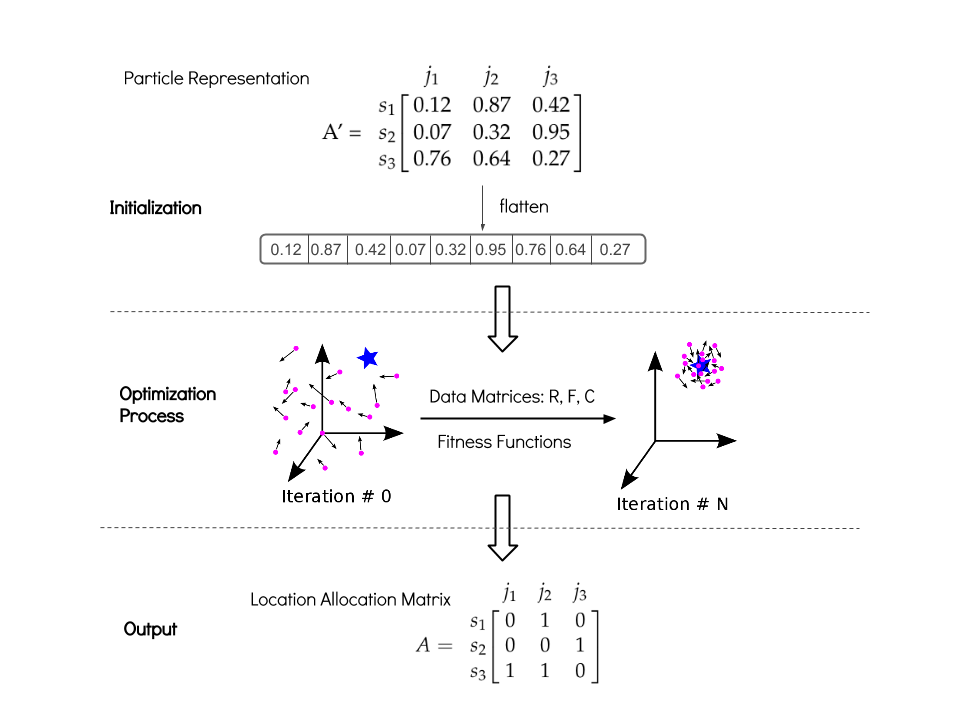
\includegraphics[width=0.9\textwidth]{./Feathergraphics/pso.png}
\end{figure}
\end{frame}
%-------------------------------------------------------
%\subsection{Required Packages}
%\begin{frame}{Installation}{Required Packages}
%-------------------------------------------------------

  %For using the Feather Theme you will need the Bemaer class installed and the following 2 packages
  %\begin{itemize}
    %\item TikZ\footnote{TikZ is a package for creating beautiful graphics. Have a look at these \chref{http://www.texample.net/tikz/examples/}{online examples} or the \chref{http://tug.ctan.org/tex-archive/graphics/pgf/base/doc/generic/pgf/pgfmanual.pdf}{pgf user manual}.}
    %\item calc
  %\end{itemize}
  %Due to the fact that the packages are very common they should be included in your latex distribution in the first place.
%\end{frame}

%-------------------------------------------------------
\subsection{Experiment Design}
\begin{frame}{Experimental Design}{}

	We designed four test cases with different complexities based on a real world dataset (WS-DREAM).
\begin{table}[h]
	{\centering
		\caption{Test Cases}
		\scalebox{0.55}{
		\begin{tabular}{|c|c|c|c|}
			\hline
			\multicolumn{1}{|l|}{problem} & \multicolumn{1}{l|}{number of service} & \multicolumn{1}{l|}{number of candidate location} & \multicolumn{1}{l|}{number of user center} \\\hline
			1                             & 20                                  & 5                                    & 10                                      \\\hline
			2                             & 50                                  & 15                                    & 20                                      \\\hline
			3                             & 100                                 & 25                                   & 40                                     \\\hline
			4                             & 200                                 & 40                                   & 80                                    \\
			\hline
		
		\end{tabular}
	}
	\\}
\end{table}

Conduct experiments on two algorithms:
\begin{itemize}
	\item Multi-objective PSO
	\item NSGA-II
\end{itemize}

\end{frame}
\subsection{Experimental Results}
%\subsection{Loading the Theme and Theme Options}

\begin{frame}{Experimental Result}{}
\begin{figure}[htb]
	\centering
	\begin{subfigure}[b]{0.6\textwidth}
	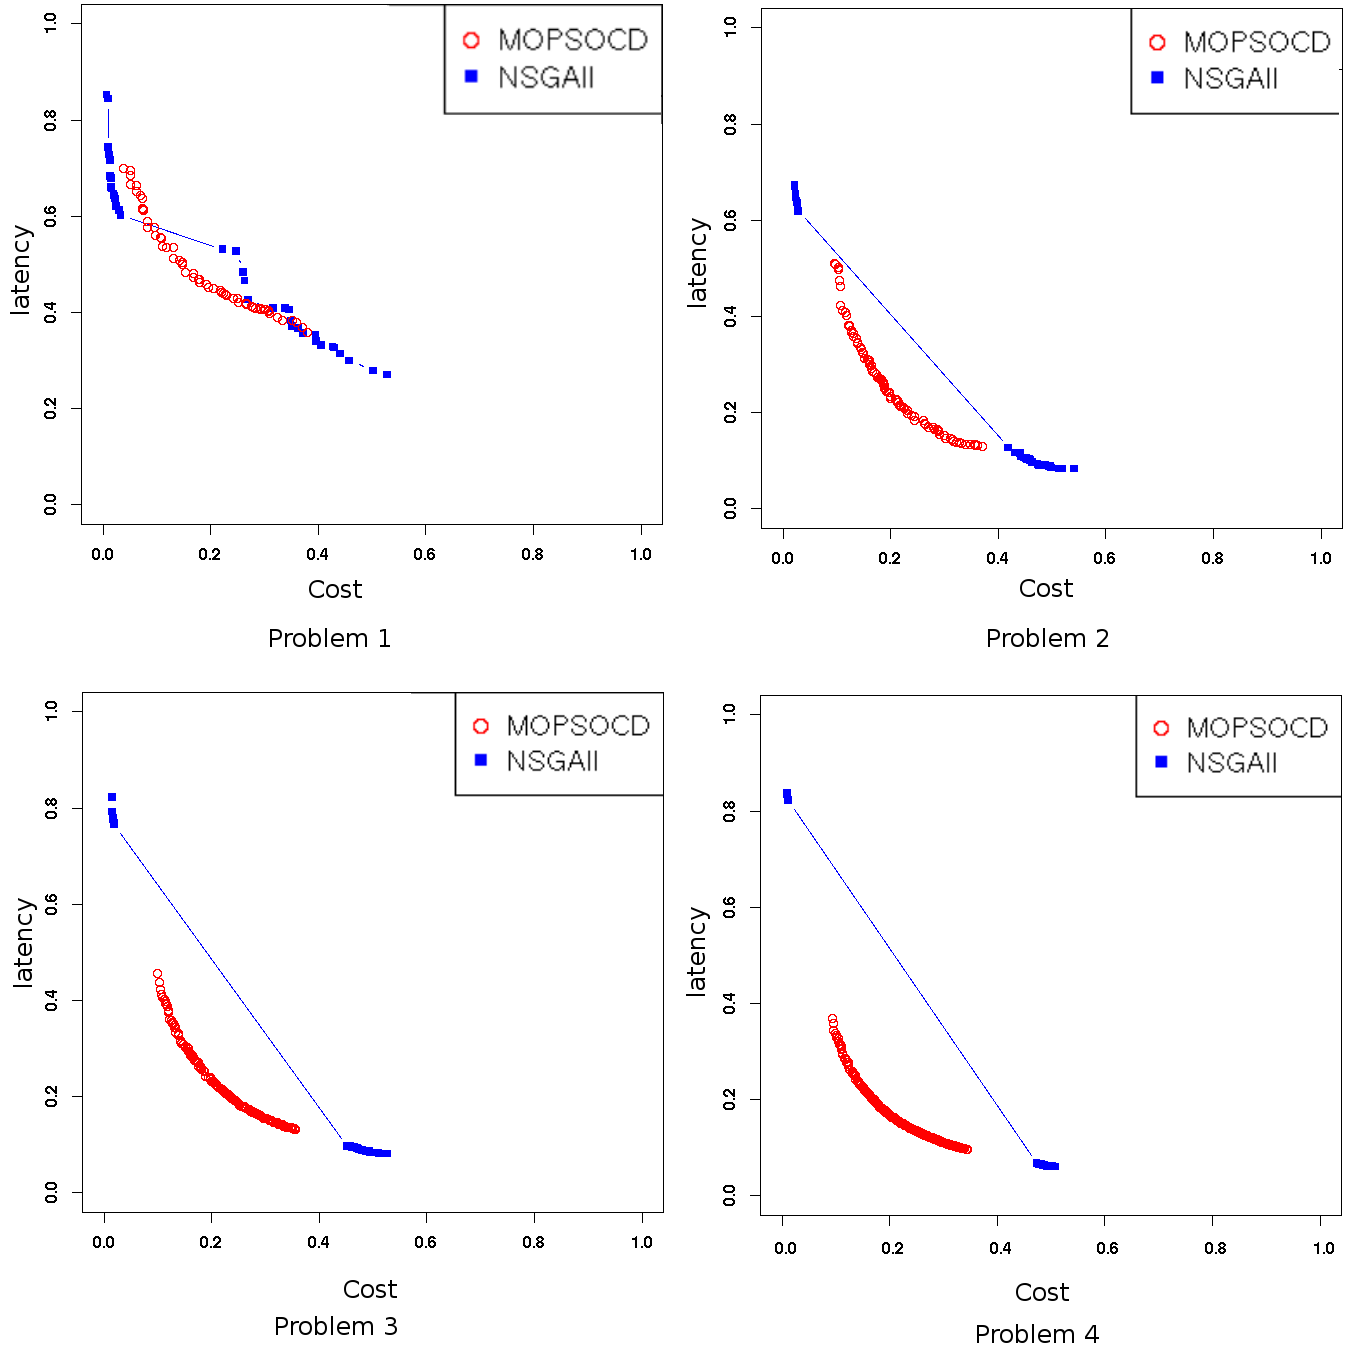
\includegraphics[width=\linewidth]{./Feathergraphics/summary.png}
	\end{subfigure}
	\begin{subfigure}[b]{0.39\textwidth}
		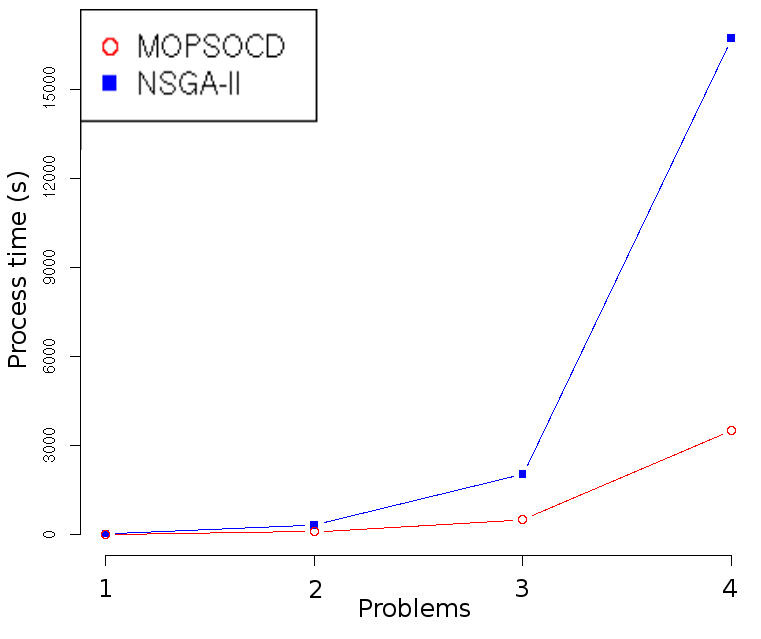
\includegraphics[width=\linewidth]{./Feathergraphics/state3.png}
	\end{subfigure}
\end{figure}
\end{frame}
%\begin{block}{Experimental Results}

%\end{block}
%-------------------------------------------------------

  %\begin{block}{The Presentation Theme}
    %The Feather Theme can be loaded in a familiar way. In the reamble of your {\tt tex} file you must type\\ \vspace{5pt} 
    %{\tt \textbackslash usetheme[<options>]\{Feather\}}\\ \vspace{5pt} 
    %The presentation theme loads the inner, outer and color Feather theme files and passes the {\tt <options>} on to these files.
  %\end{block}
  %\begin{block}{The Inner and Outher Themes}
    %If you wish you can load only the inner, or the outher theme directly by\\ \vspace{5pt} 
    %{\tt \textbackslash useinnertheme\{Feather\}} (and it has no options)\\ \vspace{5pt} 
    %{\tt \textbackslash useoutertheme[<options>]\{Feather\}} (it has one option)\\
    %\hspace{20pt}{\tt progressstyle=\{fixedCircCnt or movingCircCnt\}} \\
    %\begin{itemize}
    %\item which set how the progress is illustrated;
    %\item the value {\tt movingCircCnt} is the default.
    %\end{itemize}
  %\end{block}
%\end{frame}

%\begin{frame}{User Interface}{Loading the Theme and Theme Options}

  %\begin{block}{The Color Theme}
    %Also you can load only the color theme by writing in the preamble of the {\tt tex} file 
    
    %\vspace{5pt} 
    
    %\begin{itemize}
    %\item {\tt \textbackslash usecolortheme\{Feather\}}
    %\end{itemize}
    
    %\vspace{5pt}
    
    %...or to change the colors of the various elements in the theme
    
    %\vspace{5pt} 
    %\begin{itemize}
    %\item Change the bar colors: \\    
    %{\tt \textbackslash setbeamercolor \{Feather\}\{fg=<color>, bg=<color>\}}
    
    %\vspace{2pt} 
    
    %\item Change the color of the structural elements: \\    
    %{\tt \textbackslash setbeamercolor\{structure\}\{fg=<color>\}}
    
    %\vspace{2pt} 
    
    %\item Change the frame title text color:\\
    %{\tt \textbackslash setbeamercolor\{frametitle\}\{fg=<color>\}}
    
    %\vspace{2pt} 
    
    %\item Change the normal text color background:    
    %{\tt \textbackslash setbeamercolor\{normal text\}\{fg=<color>, bg=<color>\}}
    %\end{itemize}
  %\end{block}
%\end{frame}


%-------------------------------------------------------
%\subsection{Feather image}
%\begin{frame}{User Interface}{The Feather Background Image}
%-------------------------------------------------------

%\begin{block}{The Feather Background Image}
    %\begin{itemize}
    %\item In Feather theme, the title page frame and the last frame have the Feather image as the background image. 
    %\item The Feather background image can be produced to any frame by wrating on the begining at the choosen frame the following
    %\end{itemize} 
    
    %\vspace{5pt} 
    
  %{\tt \{\textbackslash 1bg\\
    %\textbackslash begin\{frame\}[<options>]\{Frame Title\}\{Frame Subtitle\}\\
    %\ldots\\
    %\textbackslash end\{frame\}\}}
%\end{block}
%\end{frame}


%{\1
%\begin{frame}[plain,noframenumbering]
  %\finalpage{Thank you for using Feather Beamer Theme!}
%\end{frame}}

%\section{Conclusion and Future Plan}
%\begin{frame}{Conclusion}{}
%\end{frame}
\section{Future Plan}
\begin{frame}{Future Plan}{}
	\begin{itemize}
		\item Develop a single-objective PSO and compare with Multi-objective PSO
		\item Use hypervolume and Invert Generational Distance (IGD) to analyze the parameter settings and further improve the algorithm.
	\end{itemize}


\begin{figure}[htb]
	\centering
	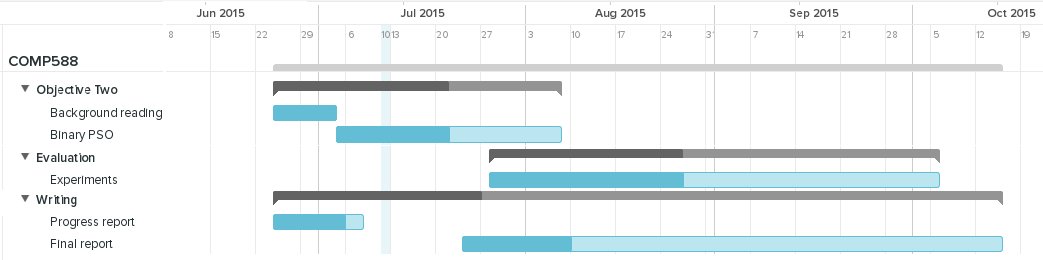
\includegraphics[width=\textwidth]{./Feathergraphics/timetable.png}
\end{figure}
\end{frame}
\end{document}
